\subsection{When is regression better than the baselines? (H6)}
\textbf{Difference in means.} In the linear one-hop model DiM estimates only the direct effect, so its bias is $-\bar\gamma$ ($-1.00$ at $\gamma=1$ under Bernoulli on every graph), independent of $n$, whereas the regression is unbiased but pays leverage $L\ge1/v$. The regression has lower RMSE than DiM only when the spillover exceeds roughly the regression's own noise floor, $\gamma^\ast\approx\hat\kappa\sqrt{L/n}$ (Fig.~\ref{fig:cross}). Across nine (degree, $n$) combinations on ER graphs, the measured crossover (RMSE ratio $=1$, log-interpolated, mean of 6 worlds) is within $0.67$--$1.02\times$ of $\hat\kappa\sqrt{L/n}$ (Table~\ref{tab:cross}). It is large for dense graphs and small samples: with $n=10^3$, $d=128$ the spillover must be $0.82\beta$ before regression helps, whereas at $n=1.6\times10^4$, $d=8$ it is $0.03\beta$. When there is no interference ($\gamma=0$) DiM is better by a factor $\sqrt{L v}=\sqrt{1+d_H}$ (RMSE $0.016$ vs $0.047$ at $d=8$, $n=1.6\times10^4$; $0.032$ vs $0.38$ at $d=128$, $n=4000$). On the real graphs the crossover is at $\gamma\approx0.07$ (Stanford3) and $\approx0.12$ (ego-Facebook) under Bernoulli design and at $\approx0.06$ and $\approx0.19$ under cluster randomization (Fig.~\ref{fig:cross}c; read off the grid $\gamma\in\{0,0.05,0.1,0.2,\dots\}$ by interpolation).

\textbf{H\'ajek.} The full-neighbourhood H\'ajek estimator is unbiased when defined but is undefined in $79\%$ of draws at $d=16$ ($n=4000$) and $100\%$ for $d\ge32$ under Bernoulli (Appendix Table~\ref{tab:cross}); where defined its RMSE is $1.3$--$1.6$ on ER. On Stanford3 and ego-Facebook, whose low-degree units supply qualifying exposures, it is defined and unbiased but has RMSE $0.48$ and $0.67$ under Bernoulli versus $0.07$ and $0.12$ for the regression; with $\approx30$ clusters it is competitive on ego-Facebook ($0.070$ vs $0.042$) and worse on Stanford3 ($0.179$ vs $0.037$). With strongly nonlinear responses and cluster randomization on ego-Facebook it matches the linear regression (threshold: $0.07$ vs $0.07$; $k{=}4$: $0.07$ vs $0.08$), so on clusterable graphs it is a safe alternative.

\begin{figure}[t]
\centering
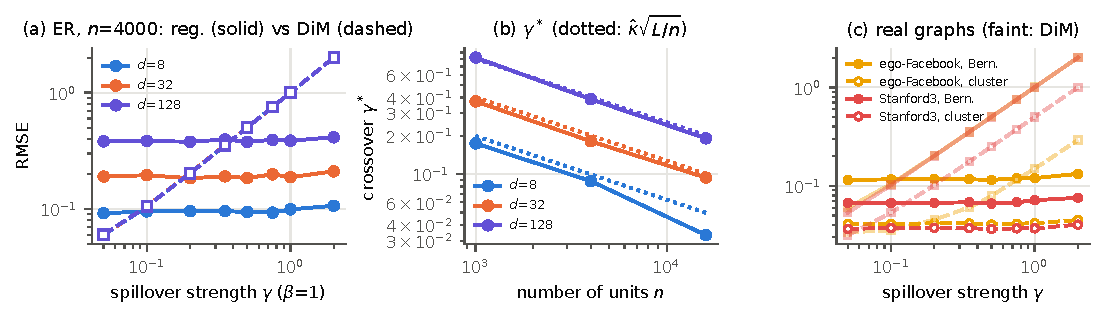
\includegraphics[width=\linewidth]{figs/fig_crossover.pdf}
\caption{Regression vs DiM (E4). (a) RMSE vs $\gamma$ on ER graphs ($n{=}4000$, $\beta{\approx}1$): regression (solid) is flat at its noise floor, DiM (dashed) grows with its bias. (b) Spillover strength at which both have equal RMSE vs $n$ for three degrees; dotted: $\hat\kappa\sqrt{L/n}$. (c) Real graphs, Bernoulli (solid) and clustered (dashed; hollow), regression in colour, DiM faint. Mean over 6 worlds.}
\label{fig:cross}
\end{figure}

\subsection{Confidence intervals}
We audit three standard errors for the one-hop regression (E6; $R=400\times6$ worlds; 8 graph/design combinations): the HC1 sandwich over units; a sandwich clustered on Louvain communities; and a graph-HAC allowing residuals of units within two hops to correlate~\citep{kojevnikov2021limit} (coverage in Appendix Fig.~\ref{fig:inf}). \emph{Correct model:} HC coverage is near nominal (mean $0.95$, range $0.87$--$1.00$ over the 48 world-settings; mean SE/SD ratio $1.03$); the clustered sandwich is slightly anticonservative ($0.93$, ratio $0.97$) and the HAC more so ($0.88$, ratio $0.91$; $0.79$ for ER with $d=30$), its 2-hop pattern covering $4\%$--$34\%$ of all pairs. \emph{Misspecified models} (concave $k=\frac12$, multi-hop $\lambda=0.4$): HC coverage has mean $0.57$ (range $0.06$--$0.83$; lowest on Stanford3 where the bias is $3.2$ SD). This is a bias problem: coverage predicted from the observed bias, SD and mean SE under a normal approximation matches the observed one with mean absolute difference $0.011$ (correlation $0.998$, 144 world-settings). The exception is clustered designs with misspecification, where the HC SE underestimates the SD (ratio $0.46$ for Stanford3/concave, $0.58$ for ego-Facebook/multi-hop; clustered sandwich $0.79$, $0.89$). No variance estimator addresses $B$: intervals cover the regression's population target, not the GATE.



\subsection{A mis-measured network}
The interference graph is itself an estimate. In E7 exposure features are computed from a graph in which a fraction $f$ of true edges is replaced by random edges (outcomes follow the true graph, linear response). Under Bernoulli designs the one-hop regression is attenuated towards the direct effect by almost exactly $f\bar\gamma$ (App.\ Fig.~\ref{fig:obs}a): bias $-0.06,-0.11,-0.22,-0.42$ for $f=0.05,0.1,0.2,0.4$ on Stanford3 (ego-Facebook, ER alike), RMSE $0.07\to0.45$. Under cluster randomization the degradation is milder in our runs (Stanford3: bias $-0.03$, RMSE $0.037\to0.087$ at $f=0.4$; ego-Facebook: bias $+0.07$, RMSE $0.042\to0.118$); we did not investigate why, and clusters were computed on the true graph, which flatters this case. The two-step model is more fragile (bias $+0.23$ at $f=0.05$ on Stanford3, Bernoulli).


